\Chapter{CRITICAL LITERATURE REVIEW}\label{sec:RevLitt}


Our research project touches upon two areas of software engineering research: \textit{mining software repositories} and \textit{software engineering expertise}. Besides these two research fields, we relied on another type of literature to conduct this research project: Git and Linux documentation. This chapter provides a critical literature review of our academic research areas and a description of the information available in the Linux and Git documentation, as well as how it helped us find solutions for the problems encoutered.



\section{Mining Software Repositories}

In addition to providing a contribution platform, \ac{SCM} systems track and save large amounts of information about changes brought to the source code. During the lifetime of the project, the \ac{SCM} acquires a large amount of data about the development of various projects. Mining software repositories researchers \textit{mine} this data for their research projects. This data can come from versin control systems, mailing list, or bug tracking systems.

Software repositories are not limited to \ac{SCM}. There are other types of software repositories that researchers mine to gather information about software projects. These repositories include bug tracking systems, mailing lists, source code, and issue tracking systems. Over the years, researchers have used mining software reporistories techniques that enabled them to research different topics of software engineering~\citep{Bird-2009}.

In the scope of our research, we used mining software repositories techniques in each different part of the project. Chapter 3 discusses two open source projects we created during this research project. The data used for both projects came from mining the Linux Kernel git repository and the Linux mailing lists. We eventually used this data for the creation of our maintainer recommendation system.

One of the difficulties often encountered by researchers in mining software repositories is the inability to link data coming from different entities of the software repository. In the case of the linux kernel, the difficulty was to link data from the mailing lists to the data from the git repository. A dificulty we addressed with an algorithm introduced in \citep{msr13jojo,jiang14}, as explained in chapter 4. 

Furthermore, \citep{armstrong} studied the difference between \textit{unicast} and \textit{broadcast} review systems. A unicast review system, like gerrit, provides an environment in which the code reviews are only sent to the author and cced people by default, but are still accessible by other developers. On the contrary, broadcast review system, like the email system used by the Linux community, shows the code reviews to each reader of the mailing list. There are advantages and disadvantages to both systems. The authors note, through an empirical study, that unicast reviews lead to less bugs in the future, but that broadcast systems allows for faster review cycles and allow beginers to learn the code base faster. 



\section{Software Engineering Expertise}
\label{sec:expertise_models}

Many different studies explored the concept of expertise in software engineering. the authors of two early studies, Expertise Browser \citep{mockus02} and Expertise Recommender\citep{McDonald}, offered the first two software engineering expertise models. McDonald et al. approach the topic from a problem solving percpective, meaning they recommend an expert that could help solving a problem. Today's developers have many different resources at their disposal for the purpose of problem solving. Stack Overflow\footnote{\url{https://stackoverflow.com/}}, a programming question answer exchange, is used by developers from around the world that are looking for solutions for complex problems. Before Stack Overflow's creation in 2008, developers did not have easy access to a large database of solutions provided by \textit{experts} from various topics. The authors of the Expertise Recommender were seeking to solve this problem by providing an architecture capable of recommending experts for given parts of the software project, for the sake of finding an expert to solve an issue. \citep{mockus02} approach the issue differently. They provide an expertise model to solve the issue of replacing or adding new experts to a distributed software engineering project. Both approaches base their measure of expertise on \textit{software change}. 
\citep{McDonald} recommends the last developer to bring change to a file as expert for that file. \citep{mockus02} improved upon this method by counting the number of changes associated to each developer to recommend an expert for each file. These software changes are the equivalent of git commits, as explained in \autoref{sec:commit_anatomy}.


Each of these previous studies ~\citep{Bhattacharya}, ~\citep{mockus02}, ~\citep{McDonald}, and~\citep{Fritz-2007} base their measures of expertise among developers on the tacit assumption that experience is acquired through development activities, such as number of lines of code contributed or the number of commits authored. The author in \citep{Fritz-2007} examined the reliability of this assumption. Through a review of the many studies in psychology on knowledge and expertise, \citep{Fritz-2007} disovered that there was not sufficient evidence that activity does determine one's knowledge. The authors conducted a quantitative study on 19 java programmer to assess the accuracy of these finding. With this study, they discovered that multiple activity related heuristics influenced developers' knowledge. These heurstics include authorship, role, work experience, and activity, which confirms the suitablility of using activity-based metrics to measure expertise. Furthermore,~\citep{Fritz-2007} mention the effect of code stability to code knolwedge, they explain that knowledge about a specific code area will degrade faster if the code area is not stable, i.e. the code is heavily modified. 

Globally, we found that the previous expertise models on the topic fail to address several important activities present in software development mentioned in~\citep{Fritz-2007}. Even though the authors give insightful advice on how developers acquire knowledge, they do not provide an expertise model capable of recommending expert for a certain code area. 

\section{The Anatomy of a Git Commit}
\label{sec:commit_anatomy}

A git commit is a fundamental concept in the scope of this research and for the understanding of git in general. The changes brought to source code by developers are contained in a \textit{commit}. If a developer is tasked to fix a bug or to create a new feature in a project, she will have to modify the source code in order to implement these changes. When a developer feels ready to share these changes, she can apply them to the repository in the form of a git commit. The changes are represented in the \textit{commit diff}, which contains the exact lines to be removed (-) or added (+) in the source code. Git uses the +/- lines to modify the repository of someone who \textit{pulled} the changes from the developer as depicted in \autoref{fig:commit_anatomy}. 

Furthermore, commits contain an array of metadata regarding the changes committed, all of which is accessible to anyone with a copy of the repository through a handful of builtin commands. For example, git log returns information about the past commits in the repository. \autoref{fig:commit_anatomy} shows one commit in the output printed by the following command: \texttt{git log -{}-pretty=fuller -{}-patch}, where the \texttt{-{}-pretty=fuller} shows more information and \texttt{-{}-patch} shows the commit diff. There are three main parts to the commit as seen in the image: the header, the  message, and the diff.

The header contains the following data points:

\begin{figure}[htb]
\centering
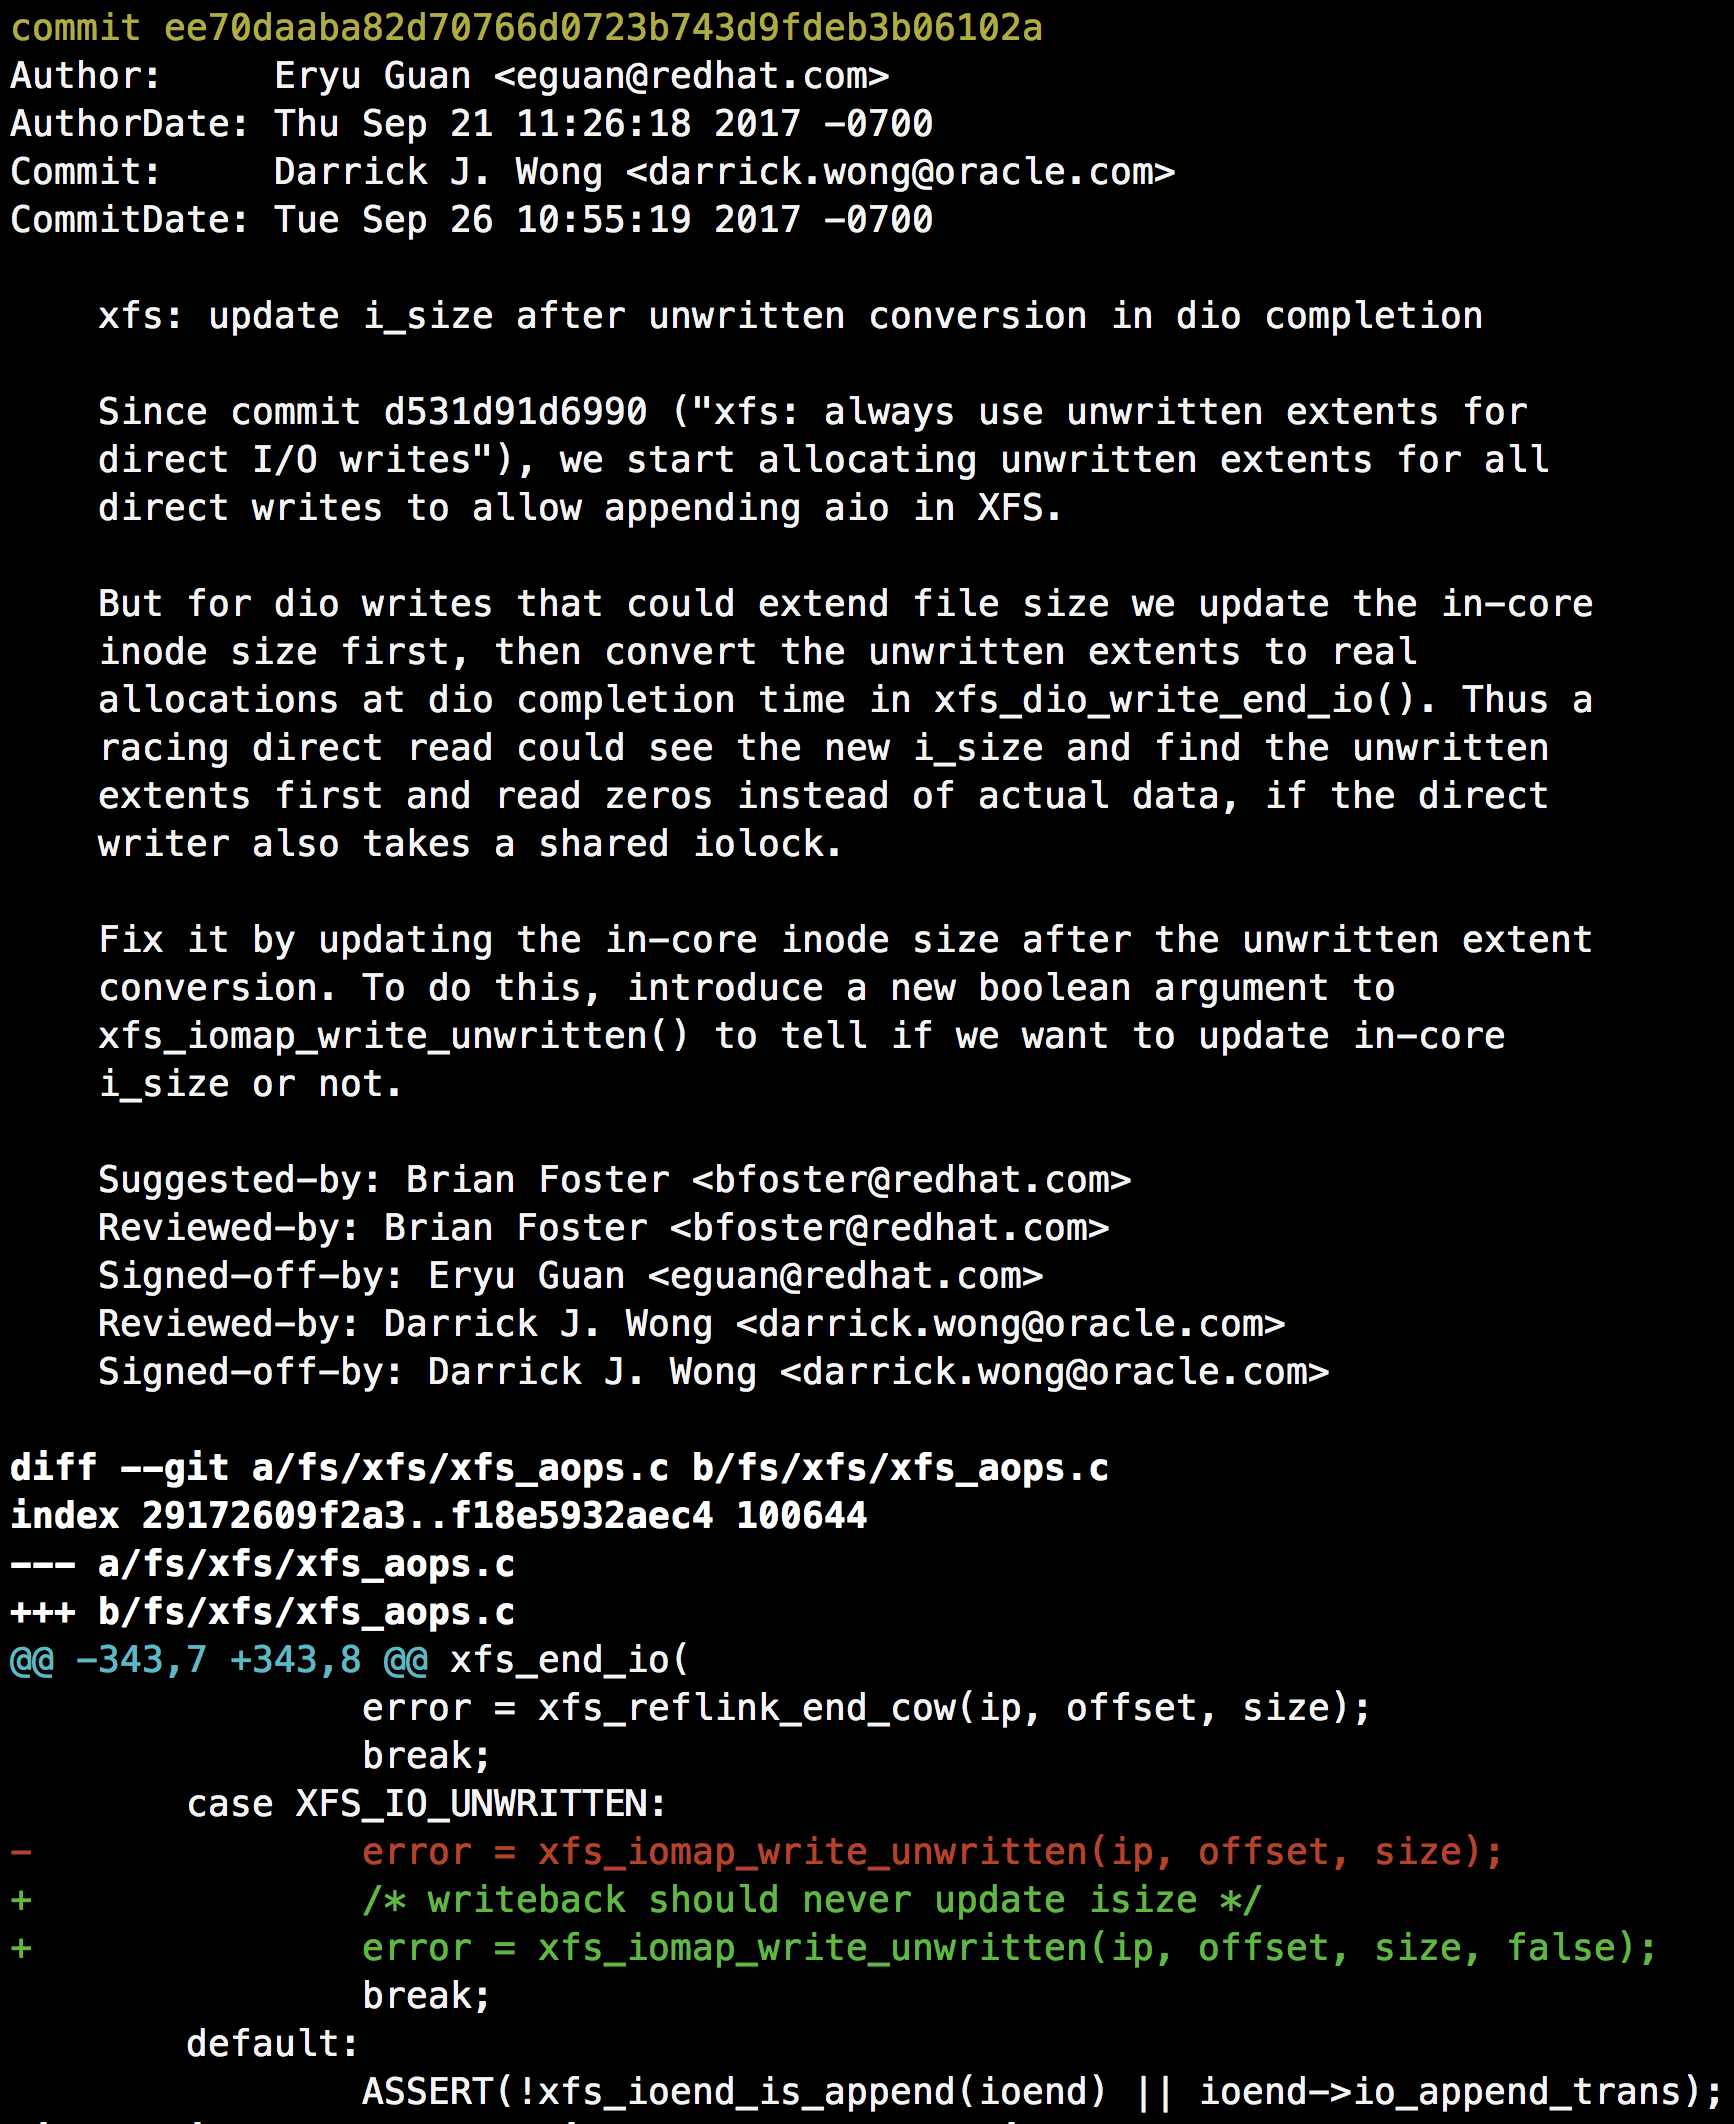
\includegraphics[width=4.5in]{commit_anatomy}
\caption{The anatomy of a commit}
\label{fig:commit_anatomy}
\end{figure}

\begin{itemize}
	\item \textbf{Commit ID:} The commit's unique identifier.
	\item \textbf{Commit Author:} Name and email address of the developer who \textit{wrote}, or \textit{authored} the code change.
	\item \textbf{Author Date:} Time, date, and timezone at which the changes were submitted.
	\item \textbf{Commit Committer:} Name and email address of the person who committed the code to the repository.
	\item \textbf{Commit Date:} Time, date, and timezone at which the commit was committed tot he repository.
\end{itemize}

In the scope of the Linux Kernel, the Commit Author rarely is the Commit Committer. As explained in \autoref{sec:Introduction}, the author is the person who wrote the code, and then submitted it for review as a patch in an email. The commit committer is the person that received, accepted, and commited the changes to their repository.

The commit message contains the following datapoints:

\begin{itemize}
	\item \textbf{Commit summary:} Often called the commit title, a brief explaination of the purpose of the commit. 
	\item \textbf{Commit Message:} In depth explanation of the purpose of the commit.
	\item \textbf{Credit Attribution Tags:} List of people who were involved in the commit and the nature of their involvement. 
\end{itemize}

There are many different types of credit attribution tags, each describing the way the person contributed to the commit. The most common ones, and the ones we use in this study are: \textit{Signed-off-by}, \textit{Reviewed-by}, and \textit{Acked-by} (acknowledged by). The tags have the following meanings\footnote{\url{https://www.kernel.org/doc/html/v4.12/process/submitting-patches.html}}. \textit{Signed-off-by} indicates the developer assisted in the creation of the patch or that she committed it upstream. \textit{Acked-by} is used by developers who were not involved in the creation of the patch but wanted to record their approval. \textit{Reviewed-by} is used to credit developers who contributed reviews to the submitted patch. 

The commit diff, which sits at the end of the git log output, shows the exact files and lines that were modified by the author of the commit. Git uses the commit diffs to apply the changes to the files in the repository. The diff can be perceived as the set of instructions to transform the source code into the desired state.



\section{Open Source Participation}

Previous work studies developers' motivation to participate in \ac{OSS}. ~\citep{Wu-oss} warn that the loosely organized nature of OSS development could be associated with a high turnover rate and in unexpected departures. Other work ~\citep{Rigby}, \citep{Foucault}, \citep{Izquierdo-Cortazar}, \citep{Mockus:2010}, \citep{Torchiano:2011:MPT:1985374.1985379}, and \citep{Ricca:2011:DCT:2022348.2022383} study the impact of a high turn over on the organization. The authors argue that departing developers leave the project with the knowledge they acquired during their time as a contributor, removing this knowledge from the project. We believe that this implies that OSS projects are at risk of knowledge loss and we believe that accurate expertise modeling could assist in addressing this issue.





